% The IF subgraph is discarded, leaving arg_1 at the free-space pointer.
\resizebox{0.78\textwidth}{!}{%
  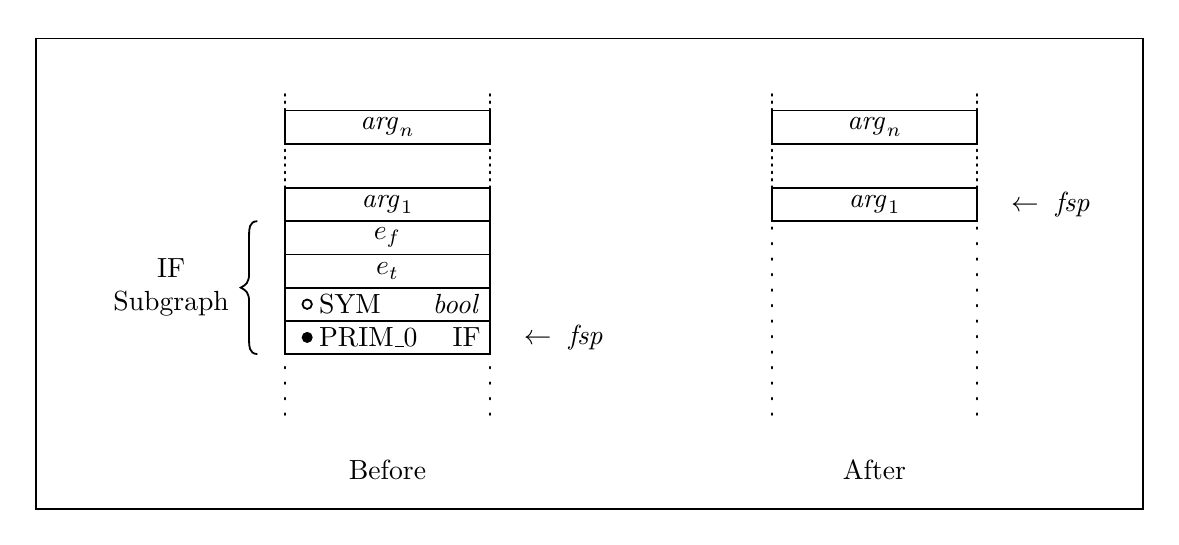
\begin{tikzpicture}[x=1pt,y=1pt,line width=0.65pt,
    font=\normalsize,inner sep=0pt,
    continuation/.style={dotted,line cap=round},
    omitted/.style={dash pattern=on 0.6pt off 5pt,line cap=round}]
    \path[use as bounding box] (-3,-3) rectangle (403,173.9293);
    \draw (0,0) rectangle (400,170);
    \foreach \x in {90,266} {
      \draw[continuation] (\x,144) -- (\x,150);
      \draw[continuation] (\x+74,144) -- (\x+74,150);
      \draw (\x,132) rectangle (\x+74,144);
      \node at (\x+37,138) {\(\mathit{arg}_n\)};
      \draw[continuation] (\x,116) -- (\x,132);
      \draw[continuation] (\x+74,116) -- (\x+74,132);
      \draw (\x,104) rectangle (\x+74,116);
      \node at (\x+37,110) {\(\mathit{arg}_1\)};
    }
    \draw (90,56) rectangle (164,104);
    \foreach \y in {68,80,92} {\draw (90,\y) -- (164,\y);}
    \node at (127,98) {\(e_f\)};
    \node at (127,86) {\(e_t\)};
    \draw (98,74) circle (1.7pt);
    \fill (98,62) circle (2pt);
    \node[anchor=west] at (102,74) {SYM};
    \node[anchor=east] at (161,74) {\(\mathit{bool}\)};
    \node[anchor=west] at (102,62) {PRIM\_0};
    \node[anchor=east] at (161,62) {IF};
    \draw[omitted] (90,34) -- (90,56);
    \draw[omitted] (164,34) -- (164,56);
    \draw[omitted] (266,34) -- (266,104);
    \draw[omitted] (340,34) -- (340,104);
    \node[anchor=west] at (176,62) {\(\leftarrow\ \mathit{fsp}\)};
    \node[anchor=west] at (352,110) {\(\leftarrow\ \mathit{fsp}\)};
    \draw (80,104) .. controls (77,104) and (77,101) .. (77,99)
      -- (77,85) .. controls (77,82) and (76,81) .. (74,80)
      .. controls (76,79) and (77,78) .. (77,75)
      -- (77,61) .. controls (77,59) and (77,56) .. (80,56);
    \node[anchor=east,align=center] at (70,80) {IF\\Subgraph};
    \node at (127,14) {Before};
    \node at (303,14) {After};
  \end{tikzpicture}%
}
